\section{Section 2: Malthusian Growth Model}
\subsection{Background}


\begin{frame}{Malthusian Growth Model}
\begin{columns}
    \begin{column}{0.6\textwidth}
        \begin{itemize}
    \item The Malthusian growth model is a mathematical model of population growth.
   \item It is essentially exponential growth of population.
   \item The model is named after Thomas  Malthus, who wrote \textit{An Essay on the Principle of Population} (1798), one of the first and most influential books on population.
  \end{itemize}
    \end{column}

    \begin{column}{0.4\textwidth}
    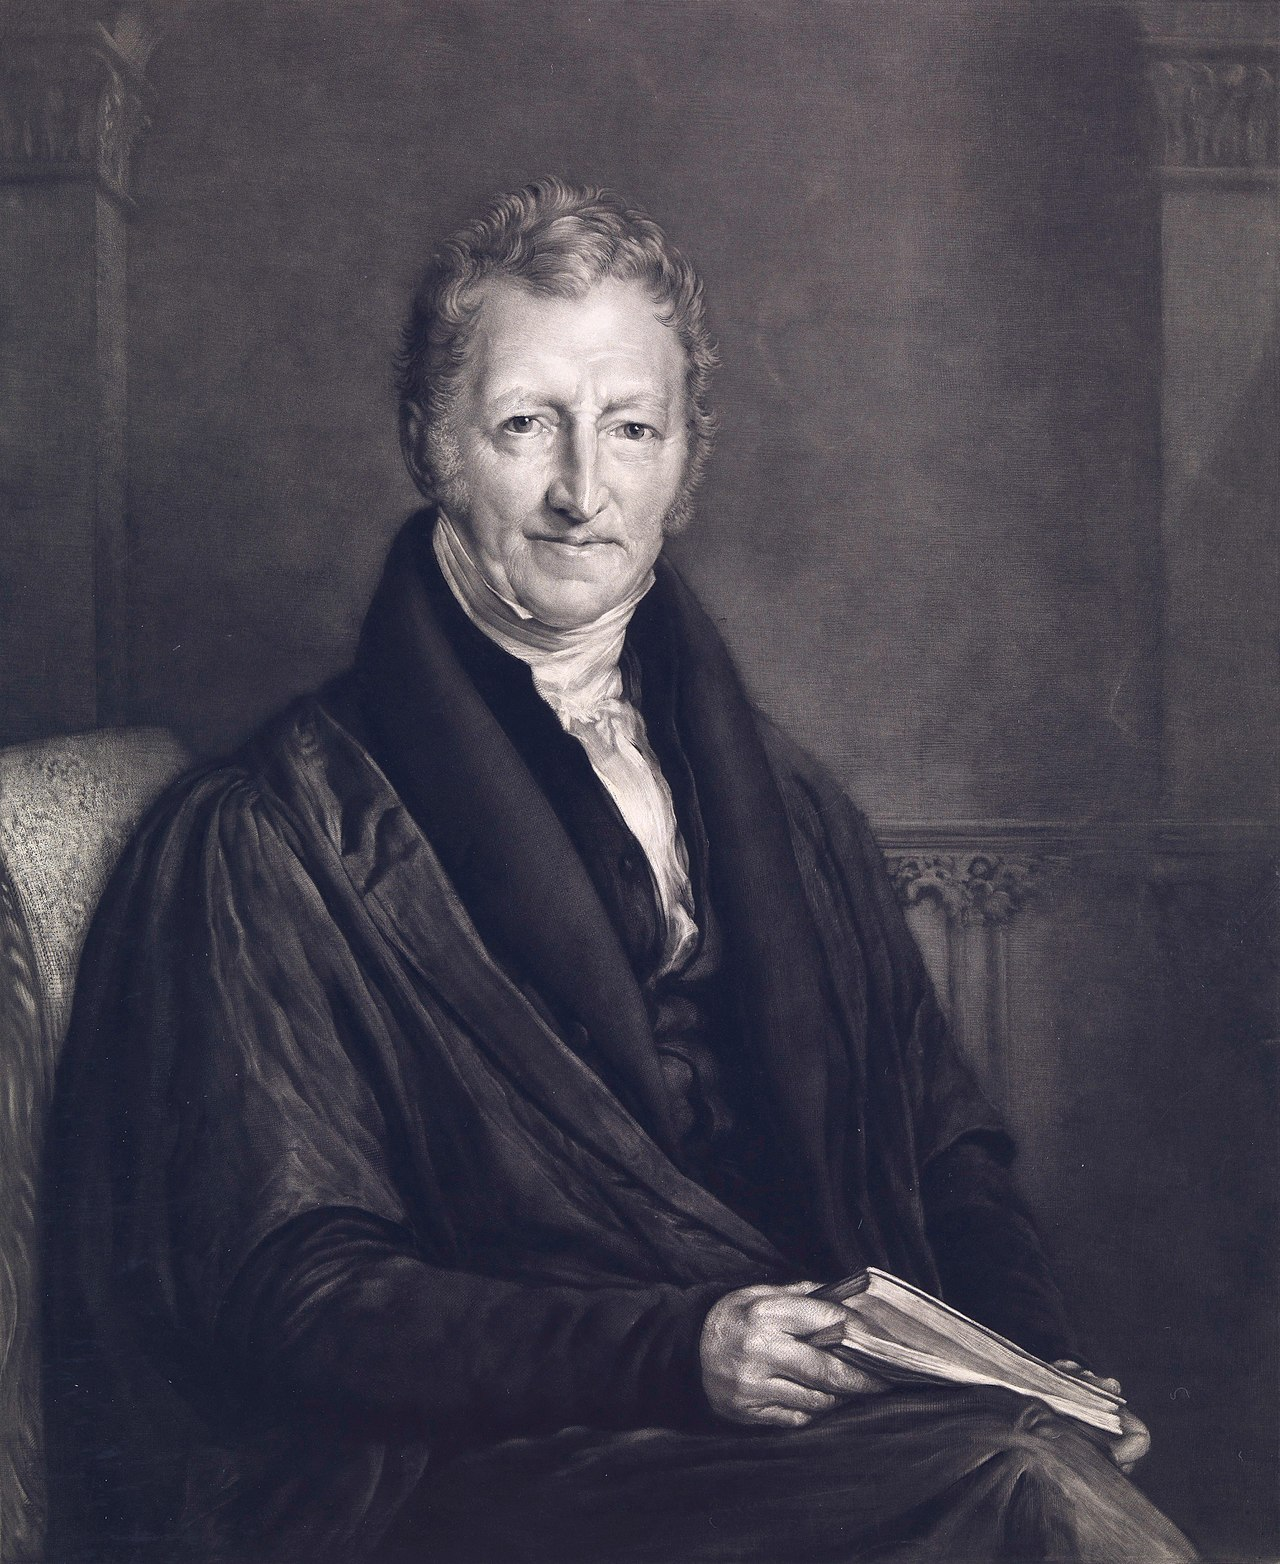
\includegraphics[scale = 0.08]
    {lesson_1/images/malthus_portrait.jpg}
       Thomas Robert Malthus 1766 - 1834, an English economist and scholar.
    \end{column}
\end{columns}
\end{frame}
  
\begin{frame}{Key assumption of  Thomas Malthus}
\begin{itemize}
    \item \textbf{Population grows exponentially when resources are abundant.}
    \item Mathus further thought that Agricultural production increases linearly.
    \item Population growth is limited by available resources and can be reduced by famine, disease, or war.
\end{itemize}
\vfill
\small

%\pause
\begin{block}{Malthusian Catastrophe}
A situation where population exceeds the agricultural production of its environment. Results in severe consequences like poverty, famine, disease, and war. Malthus believed a Malthusian catastrophe was inevitable unless population growth was controlled
\end{block}
\end{frame}


\begin{frame}{Malthus, Darwin and Natural Selection }
    \begin{itemize}
        \item Before reading Malthus, Darwin had thought that living things reproduced just enough individuals to keep populations stable
        \item Malthus helped him  to realize that as populations bred beyond their means, advantageous traits become more prevalent due to  competition for resources
        \item This led to the development of the theory of natural selection.
\end{itemize}
\vfill
%\pause

\footnotesize
\begin{center}
    \textit{In October 1838, that is fifteen months after I had begun my systematic enquiry, I happened to read for amusement Malthus on Population, and being well prepared to appreciate the struggle for existence which everywhere goes on from long-continued observation of the habits of animals and plants, \textbf{it at once struck me that under these circumstances favourable variations would tend to be preserved, and unfavourable ones to be destroyed.} The result of this would be the formation of a new species.
    \newline
    --- Charles Darwin
    }
    
\end{center}
\end{frame}

\begin{frame}{Neo-Malthusianism:}
\small
\begin{columns}
    \begin{column}{0.7\textwidth}
        \begin{itemize}
    \item A revival of Malthusian concerns in the 20\textsuperscript{th}  century, often focused on environmental limits.
\item Neo-Malthusians advocate for population control due to concerns about overpopulation, resource depletion, and environmental degradation.
\item Widely discussed in 1960s, examples is Paul Ehrlich's book \textit{The Population Bomb} (1968)
\item Their influence can be seen in family planning initiatives and advocacy for sustainability.
\item Modern environmentalism acknowledges the impact of population growth on resource use, pollution, and environmental strain.
\end{itemize}
    \end{column}
        \begin{column}{0.3\textwidth}
        
\includegraphics{lesson_1/images/malthus_population_bomb.jpg}
        
    \end{column}
\end{columns}




\end{frame}


\begin{frame}{Malthusian Growth Model Equation}

 Change in population $dP/dt$ is proportional to the current population size $P$ at time $t$. Parameter $r$ is the intrinsic rate of increase. It is difference between birth rate and death rate. 
    \begin{align*}
    \frac{dP}{dt} &= rP
  \end{align*}
\vfill
%\pause

To solve the differential equation, we separate the variables.
 We move terms with $P$ to one side and terms with $t$ to the other side.
    \begin{align*}
    \frac{dP}{P} &= rdt
  \end{align*}
\end{frame}


\begin{frame}{Malthusian Growth Model Equation}

We integrate both sides of the equation. Integration introduces a constant of integration, $C$.
   \begin{align*}
    \int \frac{dP}{P} &= \int r dt \\
    \ln|P| &= rt + C
  \end{align*}

%\pause
 We exponentiate both sides. We remove the absolute value as the population size always is positive, 
\begin{align*}
e^{\ln|P|} = e^{rt + C}  \\
P = e^{rt + C}  
\end{align*}
%\pause
The  integration constant $C$ represents initial population $P_0$. Substitution leads to the final explicit form
\begin{align*}
    P(t) &= P_0 e^{rt} 
  \end{align*}
\end{frame}

\begin{frame}[t]{Numerical vs explicit solution}
  

\begin{itemize}

    \item   Numerical and explicit solutions are two methods used to solve mathematical problems in modeling and simulation.
        
    \vspace{1em}
    
    \only<1>{
    \item  \textbf{Explicit solution} is based on an mathematical \textbf{exact} solution using algebraic equations. 
    \begin{itemize}
    \color{positive}
        \item  Provide a precise solution 
        \item Often allow for a deeper understanding of the underlying mathematical principles
    \color{negative}
        \item It can be very difficult or impossible to find explicit solution for more complex problems
    \end{itemize}
    }
    \only<2>{
    \item \textbf{Numerical solution} use \textbf{iterative methods to approximate} a solution using numerical calculations.

       \begin{itemize}
        \color{positive}
        \item  Allow solving a wider range of problems. 
        \item  Useful for problems that are difficult or impossible to solve explicitly
        \color{negative}
        \item Solutions are only approximate
        \item Solutions can be affected by calculation errors
        \item  Difficult to validate without explicit solutions or real-world data for comparison
    \end{itemize}}
\end{itemize}
\end{frame}

\begin{frame}{Numerical vs explicit solution for Malthusian growth}
\footnotesize

\begin{columns}
    \begin{column}{0.45\textwidth}
       \textbf{explicit Solution}
       
       Calculation using formula:
       \begin{equation*}
    P(t) = P_0 e^{rt} 
  \end{equation*}

  where 
\begin{itemize}
    \item $P_0$ is the initial population at time $0$
    \item $r$ is the growth rate
    \item $t$ is the time
\end{itemize}

        
    \end{column}
    
    %\pause
  \hspace{1em}
\vrule{}
  \hspace{1em}

    \begin{column}{0.45\textwidth}
   \textbf{Equation for numerical solution:}  
   \begin{equation*}
   \frac{dP}{dt} = rP 
\end{equation*}

\vspace{1em}
  Solution by Euler's Method:
 \begin{enumerate}
     \item  \textbf{Discretization:}
     \begin{equation*}
         t_i = i \Delta t
     \end{equation*}
        \item  \textbf{Iteration:}
     \begin{equation*}
         P(t_{i+1}) = P(t_i) + rP(t_i) \Delta t
     \end{equation*}
 \end{enumerate}
where 
\begin{itemize}
    \item $P(t_i)$ is the population at time $t_i$
    \item $r$ is the growth rate
    \item $\Delta t$ is the time step
\end{itemize}
    \end{column}
\end{columns}
\end{frame}




\subsection{Exercises}

\begin{frame}{Task 2.1:  Population at discrete times}
        
\begin{columns}
    \begin{column}{0.6\textwidth}
Calculate population at certain times of interest using explicit formula. 
\begin{itemize}
\item Initial population size: 2.5 million
\item Yearly growth rate: 2.7\%
\item Equation $P(t) = P_0 e^{rt} $ 
\item Time in years :
    \begin{itemize}
        \item 1 
        \item 5
        \item 7.6
        \item 25.78
    \end{itemize}
\item Note: Population size and growth rate correspond to population of Senegal in 1950.
\end{itemize}
    \end{column}

    \begin{column}{0.4\textwidth}
    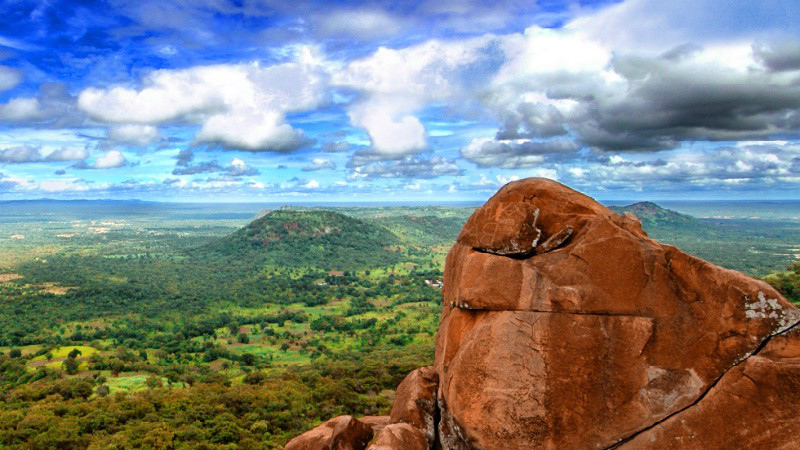
\includegraphics[scale = 0.2]{lesson_1/images/malthusian_senegal.jpeg}
\end{column}
\end{columns}


\end{frame}

\begin{frame}[fragile]{Solution 2.1: Population at discrete times}

\small
\lstinputlisting{lesson_1/code/task_2_1_malthusian_explicit_discrete.m}
\end{frame}

\begin{frame}[fragile]{Solution 2.1: Population at discrete times}
\begin{itemize}
    \item The results show population size at times of 1, 5, 7.5, and 25.78 years.
    \item The explicit solution allows us to easily calculate population predictions at any given time.  
\end{itemize}

\vfill 
\small
\begin{lstlisting}
Years of interest:
    1.0000    5.0000    7.5000   25.7800
Calculated population size:
    2.5684    2.8613    3.0612    5.0146
\end{lstlisting}

\vfill
Note: this line leads to the same result, but it is much better to maintain your code well organized. 
\begin{lstlisting}
2.5*exp(0.027*[1,5,7.5,25.78])
\end{lstlisting}

\end{frame}


\begin{frame}{Task 2: Continuous modeling with explicit solution }
\begin{itemize}
    \item The population has same parameters as in Task 1
    \item Calculate population for the next 70 years 
    \item The time step is 1 year.
    \item Plot the results.
\end{itemize}
\end{frame}

\begin{frame}[fragile]{Solution 2.2: Continuous modeling with explicit solution } 
\only<1>{
\footnotesize
\lstinputlisting{lesson_1/code/task_2_2_malthusian_explicit.m}
}
\only<2>{
    Population increase exponentially. 
    \begin{center}
    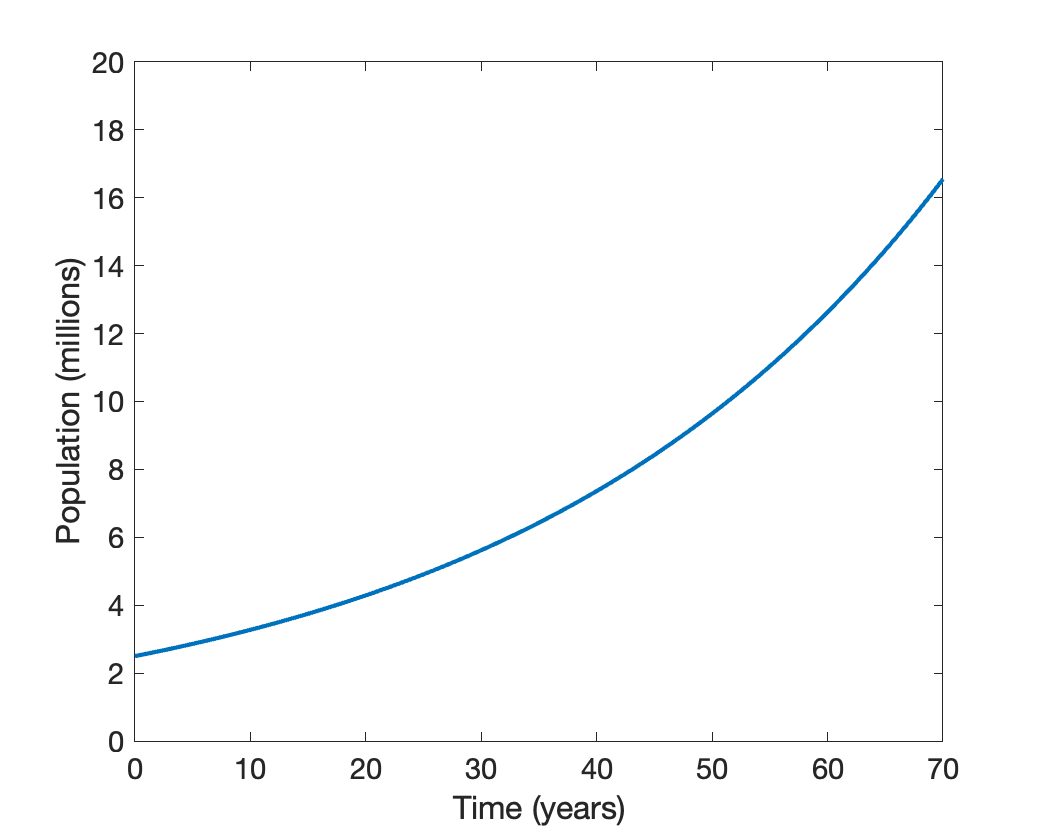
\includegraphics[scale = 0.35]{lesson_1/images/task_2_2_malthusian_explicit.png}  
    \end{center}
    }
\end{frame}




\begin{frame}{Task 2.3: Numerical approach }
    \begin{itemize}
        \item  Use numerical approach to calculate population for 0 to 70 years 
        \item The time step should be 1 year.
        \item  Plot the result.
    \end{itemize}
\end{frame}

\begin{frame}[fragile]{Solution 2.3:  Numerical approach } 
\only<1>{
\footnotesize
\lstinputlisting{lesson_1/code/task_2_3_malthusian_numerical.m}
}
\only<2>{
\begin{center}
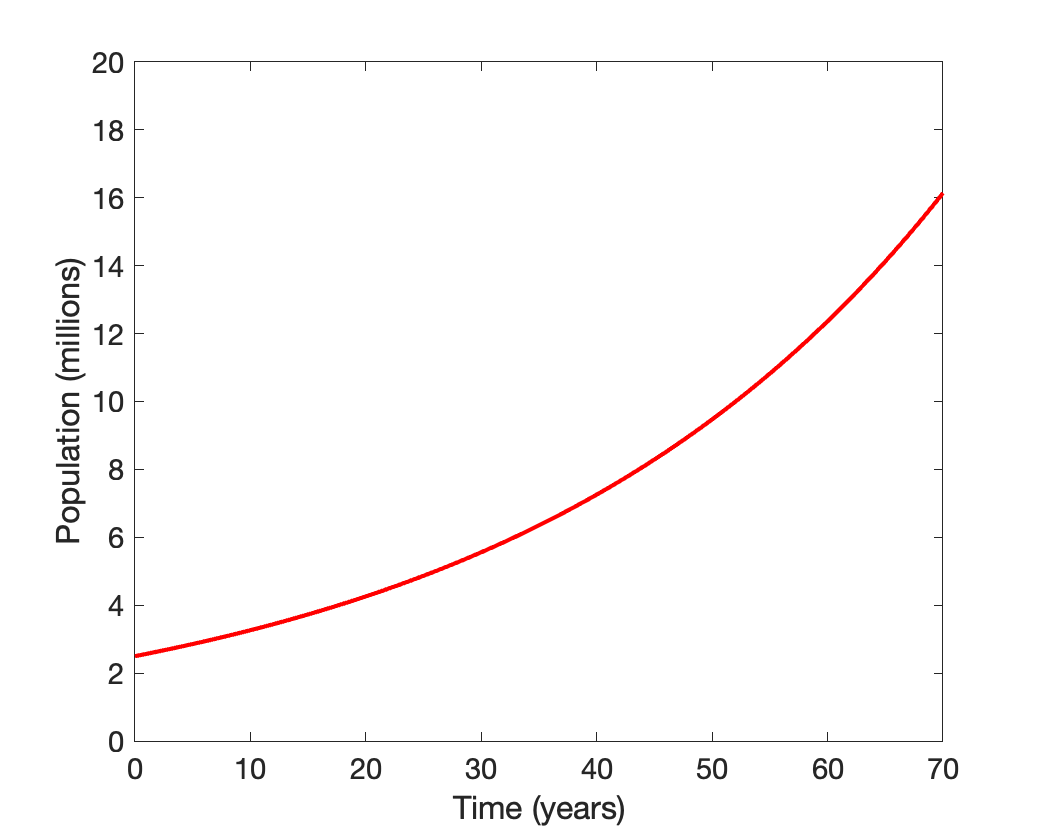
\includegraphics[scale = 0.35]{lesson_1/images/task_2_3_malthusian_numerical.png}  
\end{center}
}
\end{frame}


\begin{frame}{Task 2.4: Difference in solutions}
\begin{itemize}
    \item Create plot that shows results from explicit and numerical approach and their difference. 
    \item Add start year of 1950 to the plot to have correct timeline
    \item Compare the difference for time step of 1 year, 1 month and 1 day.
\end{itemize}

\end{frame}

\begin{frame}[fragile]{Solution 2.4: The difference in solutions} 
\only<1>{
\tiny
\lstinputlisting{lesson_1/code/task_2_4_malthusian_difference.m}
}

\begin{center}  
\only<2>{

    Step size of 1 year (70 iterations) leads to substantial error.
        \vfill
             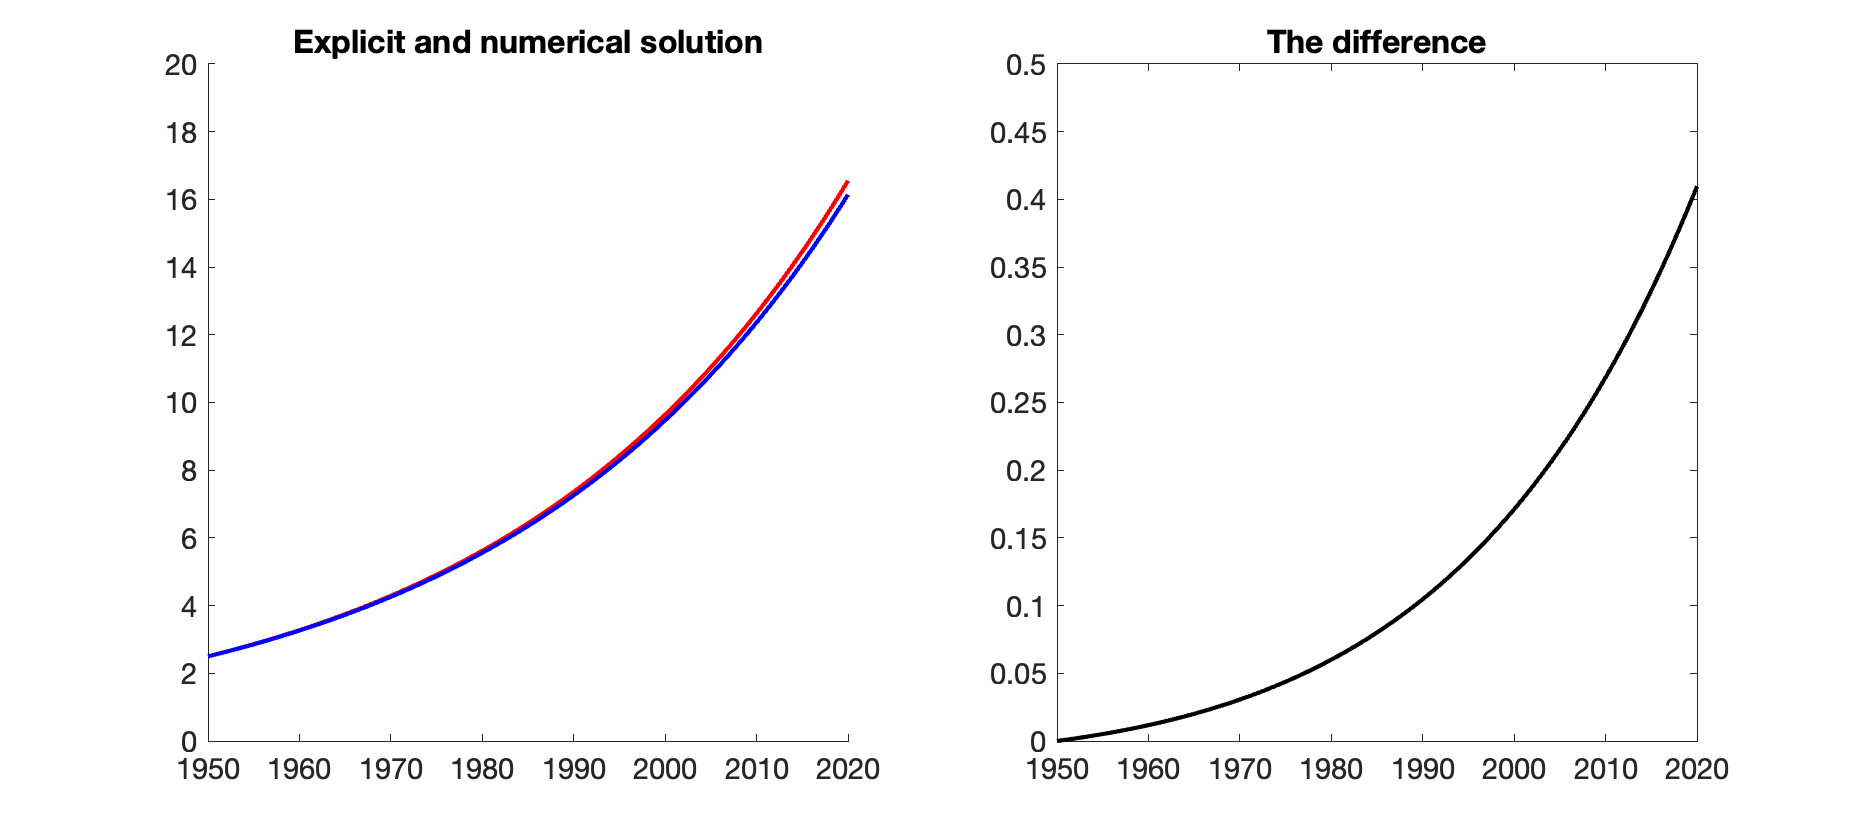
\includegraphics[scale = 0.35]{lesson_1/images/task_2_4_malthusian_difference.png}
 }
  
\only<3>{
  Step size of 1 month (840 iterations) reduces the error
      \vfill
    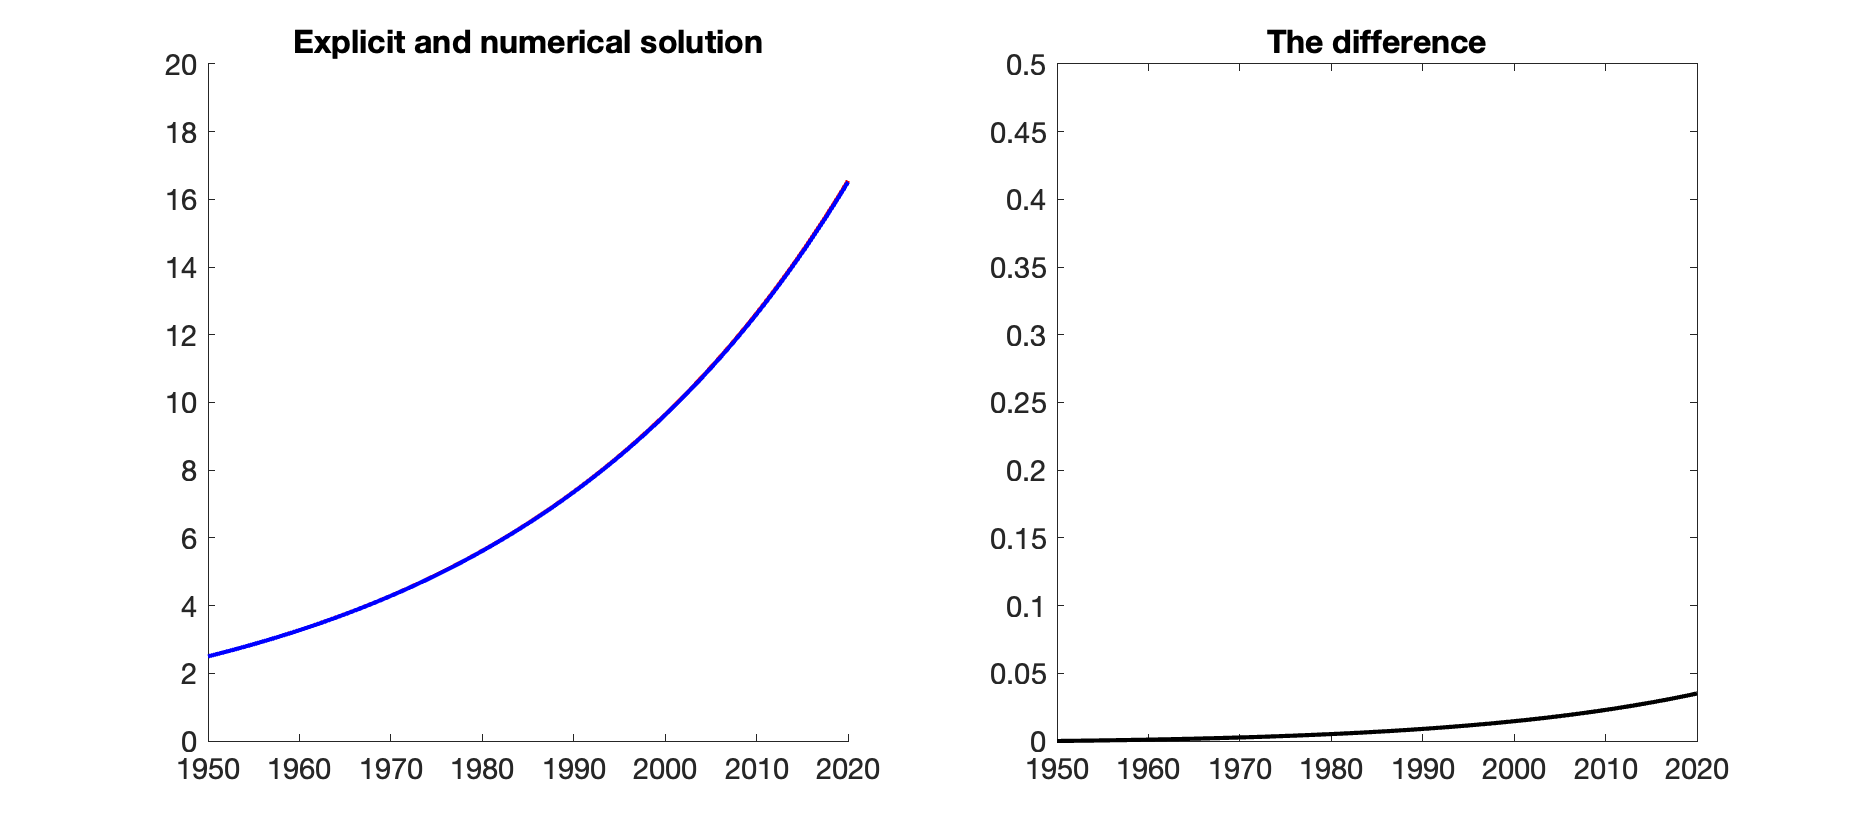
\includegraphics[scale = 0.35]{lesson_1/images/task_2_4_malthusian_difference_1month.png} 
    }
\only<4>{
    Step size of 1 day (25 550 iterations) leads to negligible error.
    \vfill
    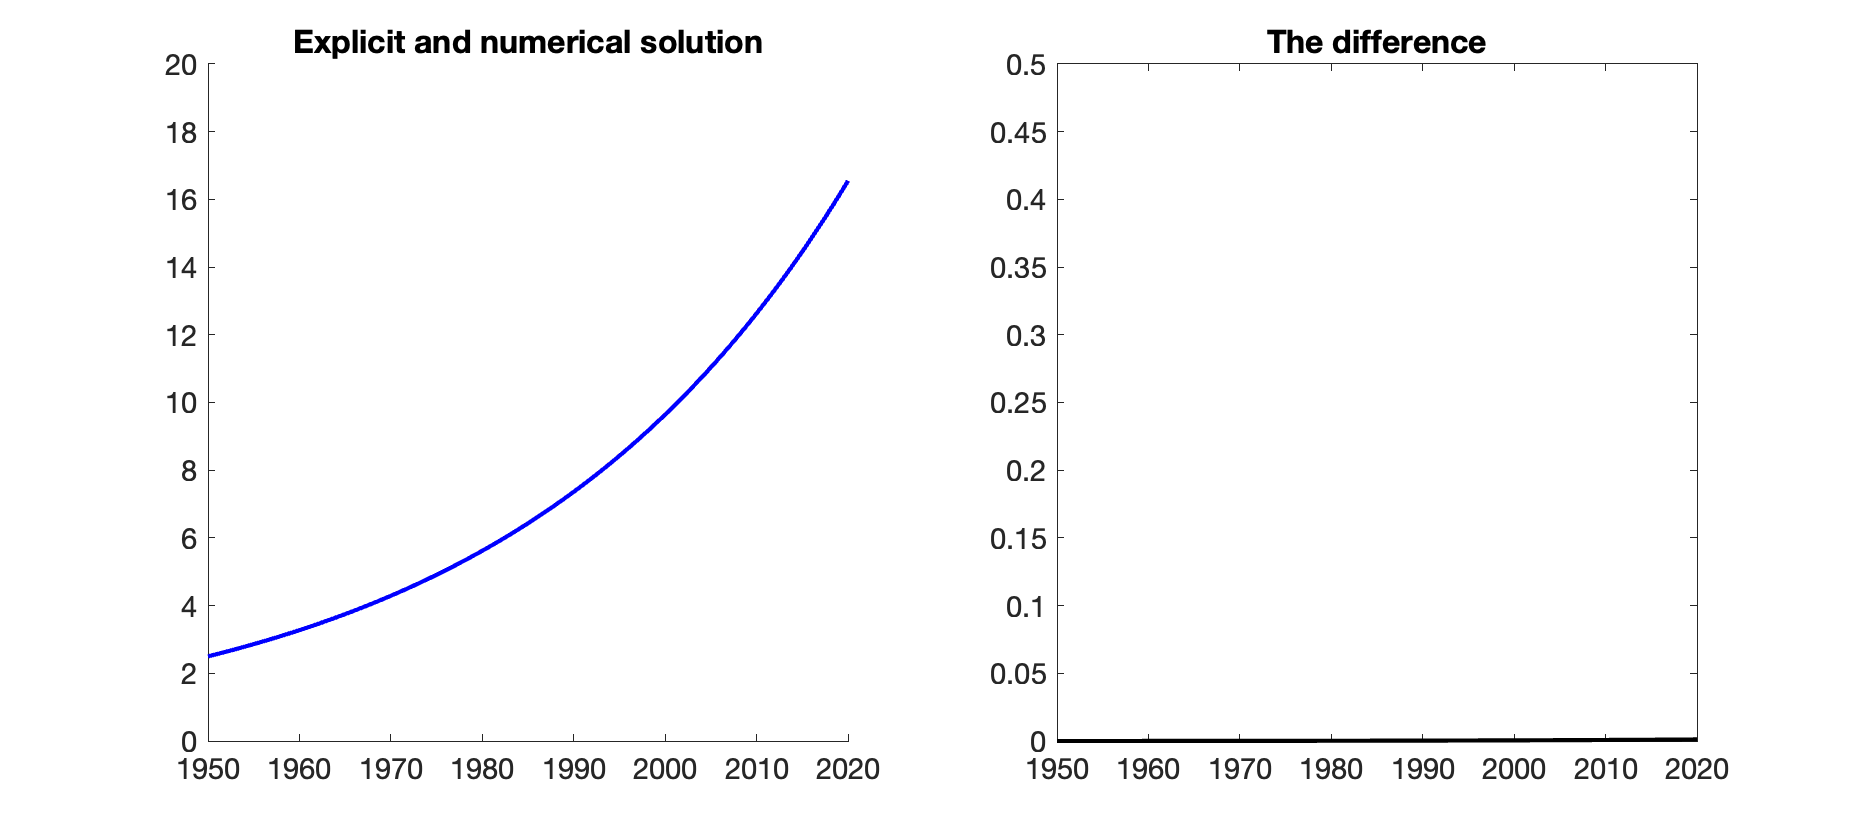
\includegraphics[scale = 0.35]{lesson_1/images/task_2_4_malthusian_difference_1day.png} 
    }
\end{center}
    
\end{frame}

\begin{frame}[fragile]{Task 2.5: Real world data}
    Compare prediction modeled by the explicit formula with real data of Senegalese population 
    \vfill
\scriptsize
\lstinputlisting[firstline=1,  lastline=13]
{lesson_1/code/task_2_5_malthusian_senegal.m}
\end{frame}


\begin{frame}[fragile]{Solution 2.5: Real world data}
\only<1>{
\tiny
\lstinputlisting{lesson_1/code/task_2_5_malthusian_senegal.m}
}
\only<2>{
Even a very simple model can be capture reality very well. 
\begin{center}
    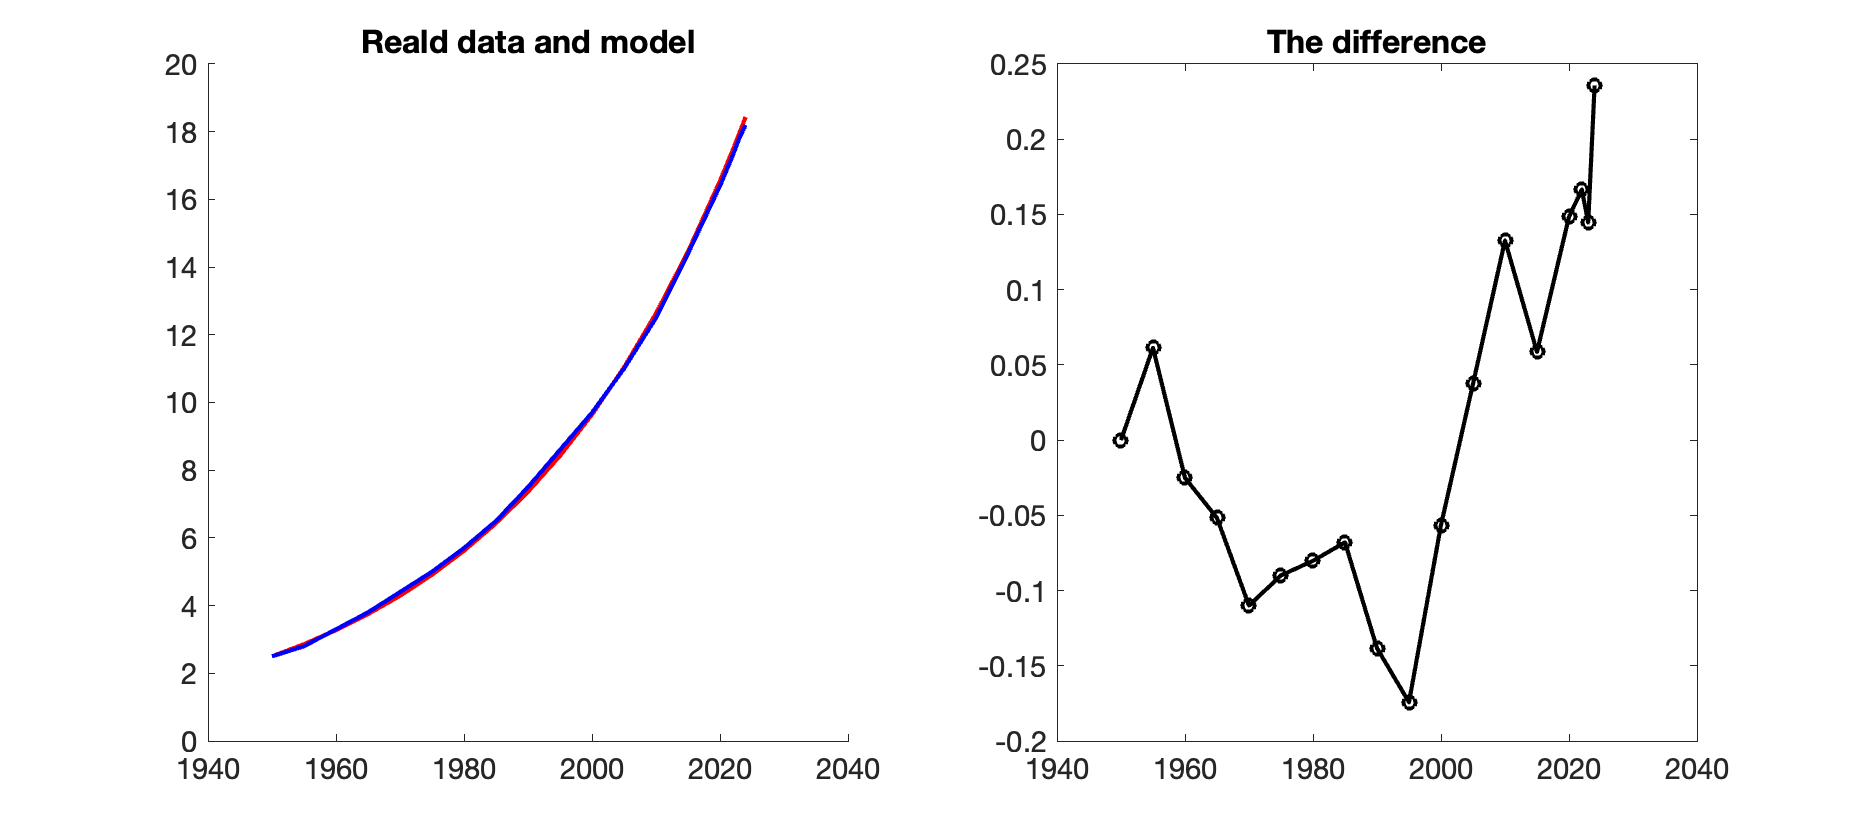
\includegraphics[scale=0.35]
{lesson_1/images/task_2_5_malthusian_senegal.png}
\end{center}

}
\end{frame}


\begin{frame}[fragile]{Task 2.6: Real world data --- USA}
\small
\begin{itemize}
    \item Compare prediction modeled by the explicit formula for USA with real data.
    \item Adjust time span start year and the initial population
    \item Set growth rate to 2.75\%.
\end{itemize}

\vfill
\tiny
\lstinputlisting[firstline=1, lastline=13]{lesson_1/code/task_2_6_malthusian_usa.m}
\end{frame}

\begin{frame}[fragile]{Solution 2.6: Real world data --- USA}
\only<1>{
\tiny
\lstinputlisting{lesson_1/code/task_2_6_malthusian_usa.m}
}
\only<2>{
Model is reasonably precise for the first one hundered years, then it diverges. \newline
\textbf{Why?}
\begin{center}
    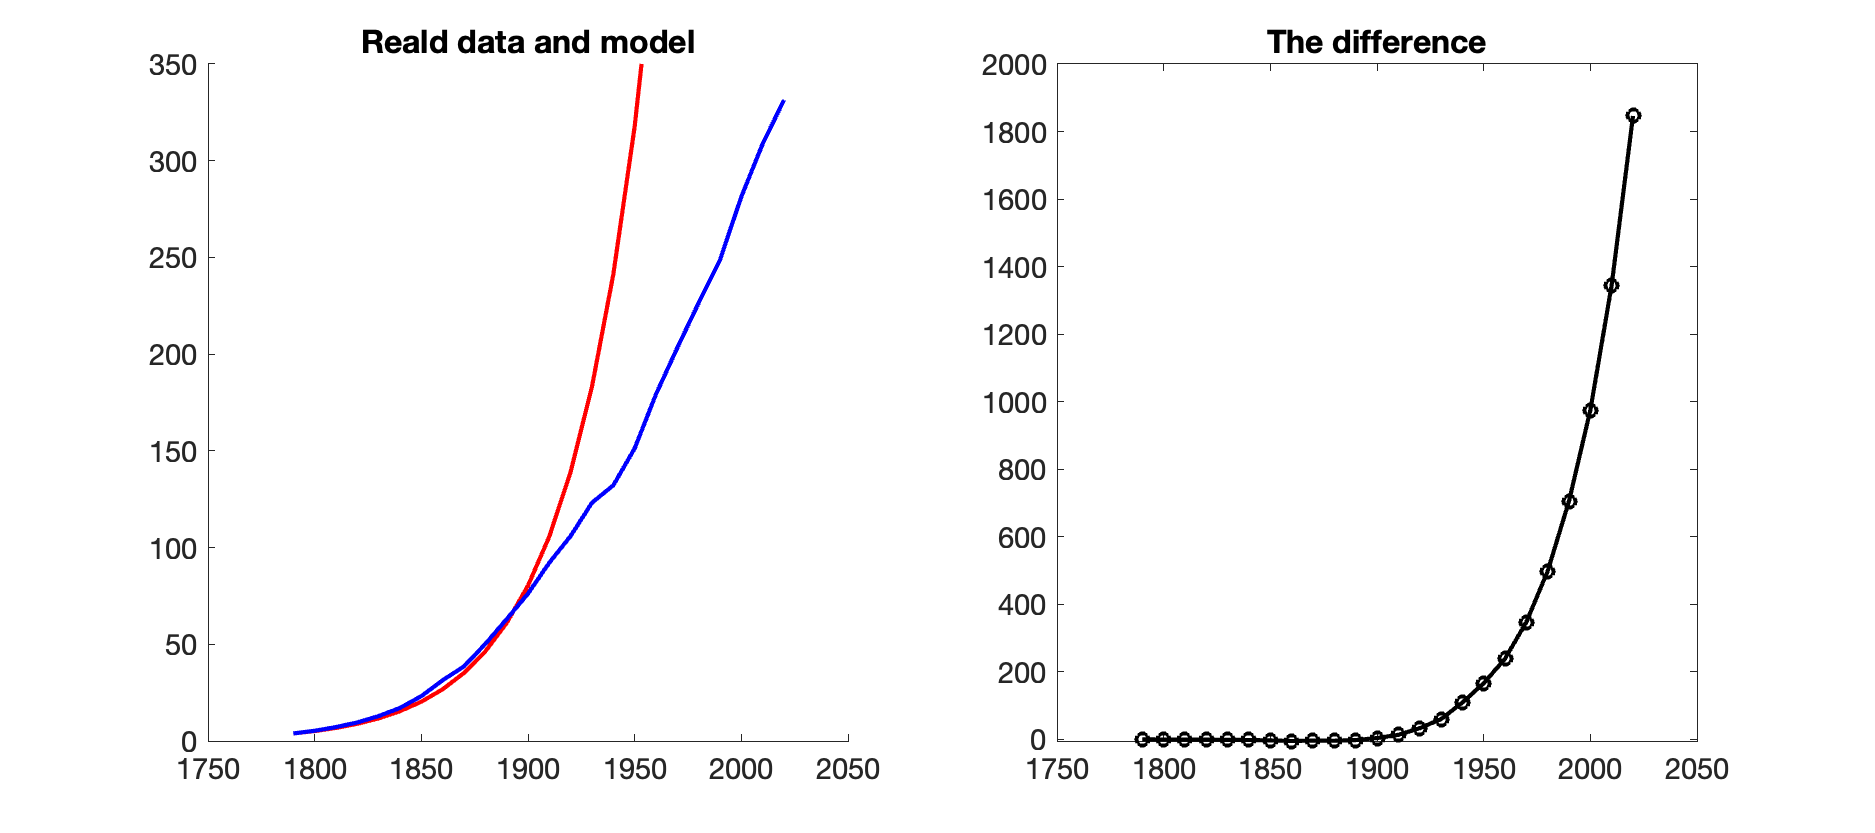
\includegraphics[scale=0.35]{lesson_1/images/task_2_6_malthusian_usa.png}
\end{center}
}
\end{frame}
